% !TeX root = ../../infdesc.tex
\section{Sets}
\secbegin{secSets}


\begin{exercise}
Which of the following propositions are true, and which are false?
\[ \frac{1}{2} \in \mathbb{Z} \qquad \frac{1}{2} \in \mathbb{Q} \qquad \mathbb{Z} \in \mathbb{Q} \qquad \mathbb{Z} \in \mathcal{U} \qquad \frac{1}{2} \in \mathcal{U} \]
\hintlabel{exElementsOfSets}{%
Think about what `$a \in X$' \textit{really means}---don't let your intuition fool you.
}
\end{exercise}


\begin{exercise}
\label{exDyadicRatioal}
\index{rational number!dyadic}
A \textbf{dyadic rational} is a rational number that can be expressed as an integer divided by a power of $2$. Express the set of all dyadic rationals using set-builder notation.
\end{exercise}


\begin{exercise}
Express the set of dyadic rationals (defined in \Cref{exDyadicRatioal}) in this alternate form of set-builder notation.
\end{exercise}

\begin{exercise}
For each of the following illustrations, find the interval that it depicts. A filled circle $\bullet$ indicates that an end-point is included in the interval, whereas a hollow circle $\circ$ indicates that an end-point is not included in the interval.

\begin{enumerate}[(a)]
\item
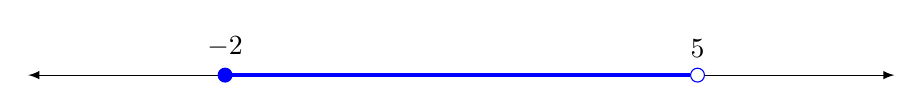
\begin{tikzpicture}
\draw[latex-latex] (-5.5,0) -- (5.5,0);
\draw[line width=1.5pt, color=blue] (-3,0) -- (3,0);
\filldraw[blue](-3,0)circle[radius=2.5pt];
\filldraw[white](3,0)circle[radius=2.5pt];
\draw[blue](3,0)circle[radius=2.5pt];
\node[at={(-3,3pt)},above]{$-2$};
\node[at={(3,3pt)},above]{$5$};
\end{tikzpicture}

\item
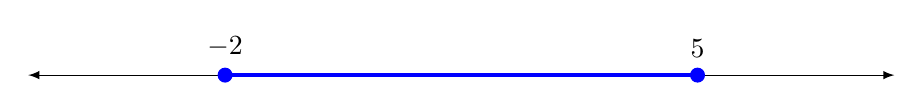
\begin{tikzpicture}
\draw[latex-latex] (-5.5,0) -- (5.5,0);
\draw[line width=1.5pt, color=blue] (-3,0) -- (3,0);
\filldraw[blue](-3,0)circle[radius=2.5pt];
\filldraw[blue](3,0)circle[radius=2.5pt];
\node[at={(-3,3pt)},above]{$-2$};
\node[at={(3,3pt)},above]{$5$};
\end{tikzpicture}


\item
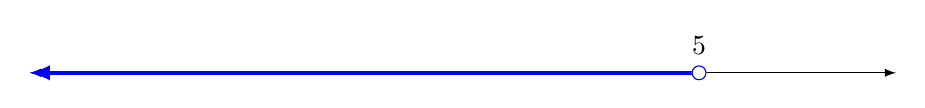
\begin{tikzpicture}
\draw[latex-latex] (-5.5,0) -- (5.5,0);
\draw[latex-, line width=1.5pt, color=blue] (-5.5,0) -- (3,0);
\filldraw[white](3,0)circle[radius=2.5pt];
\draw[blue](3,0)circle[radius=2.5pt];
\node[at={(3,3pt)},above]{$5$};
\end{tikzpicture}

\item 
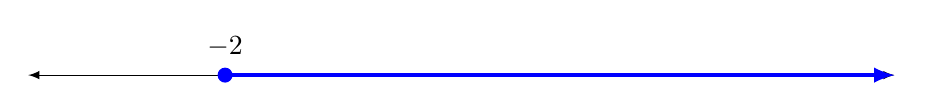
\begin{tikzpicture}
\draw[latex-latex] (-5.5,0) -- (5.5,0);
\draw[-latex, line width=1.5pt, color=blue] (-3,0) -- (5.5,0);
\filldraw[blue](-3,0)circle[radius=2.5pt];
\node[at={(-3,3pt)},above]{$-2$};
\end{tikzpicture}
\end{enumerate}
\end{exercise}


\begin{exercise}
Let $a,b,c,d \in \mathbb{R}$ with $a<b$ and $c<d$. Prove that $[a,b) \subseteq (c,d]$ if and only if $a > c$ and $b \le d$.
\end{exercise}


\begin{exercise}
Prove that $\{ x \in \mathbb{R} \mid x^2 < x \} = (0,1)$.
\end{exercise}


\begin{exercise}
Prove by double containment that $\{ 0, 1 \} = \{ 1, 0 \}$ and $\{ 0, 0 \} = \{ 0 \}$.
\end{exercise}


\begin{exercise}
Let $a,b \in \mathbb{R}$. Prove that $[a,b]$ is empty if and only if $a > b$, and that $(a,b)$ is empty if and only if $a \ge b$.
\end{exercise}


\begin{exercise}
Let $E$ be an empty set and let $p(x)$ be a predicate with one free variable $x$ with domain of discourse $E$. Show that the proposition $\forall x \in E,\, p(x)$ is true, and that the proposition $\exists x \in E,\, p(x)$ is false. What does the proposition $\forall x \in E,\, x \ne x$ mean in English? Is it true?
\hintlabel{exEverythingIsTrueOfElementsOfEmptySet}{%
Recall from the beginning of \Cref{secSets} that $\forall x \in X,\, p(x)$ is equivalent to $\forall x,\, (x \in X \Rightarrow p(x))$ and $\exists x \in X,\, p(x)$ is equivalent to $\exists x,\, (x \in X \wedge p(x))$. What can be said about the truth value of $x \in E$ when $E$ is empty?
}
\end{exercise}


\begin{exercise}
\label{exEmptySetSubsetOfEverySet}
Let $X$ be a set. Prove that $\varnothing \subseteq X$.
\end{exercise}


\begin{exercise}
Write out the elements of $\mathcal{P}(\{1, 2, 3\})$.
\end{exercise}

\begin{exercise}
Let $X$ be a set. Show that $\varnothing \in \mathcal{P}(X)$ and $X \in \mathcal{P}(X)$.
\end{exercise}

\begin{exercise}
Write out the elements of $\mathcal{P}(\varnothing)$, $\mathcal{P}(\mathcal{P}(\varnothing))$ and $\mathcal{P}(\mathcal{P}(\mathcal{P}(\varnothing)))$.
\end{exercise}


\begin{exercise}
Determine, with proof, whether or not each of the following statements is true.
\begin{enumerate}[(a)]
\item $\mathcal{P}(\varnothing) \in \mathcal{P}(\mathcal{P}(\varnothing))$;
\item $\varnothing \in \{ \{ \varnothing \} \}$;
\item $\{ \varnothing \} \in \{ \{ \varnothing \} \}$;
\item $\mathcal{P}(\mathcal{P}(\varnothing)) \in \{ \varnothing, \{ \varnothing, \{ \varnothing \} \} \}$.
\end{enumerate}
Repeat the exercise with all instances of `$\in$' replaced by `$\subseteq$'.
\end{exercise}
